\question{Автоэлектронная эмиссия. Уравнение Фаулера-Нордгейма}
Явление автоэлектронной эмиссии заключается в испускании электронов с
поверхности вещества под действием внешнего электрического поля. В его основе
лежит туннельный эффект -- пересечение электроном потенциального барьера.

Рассмотрим плоский вакуумный диод, катод которого имеет температуру вблизи
абсолютного нуля, а поле однородно. В катоде энергия электронов не
превышает энергию Ферми.
%\begin{figure}
%\begin{center}
    %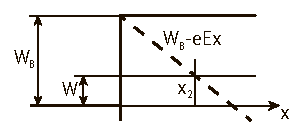
\includegraphics[width=.47\textwidth]{04}
%\end{center}
%\caption{Потенциальный барьер влизи поверхности катода}
%\end{figure}


Прозрачность барьера \( D \) для электрона с энергией \( W \) пропорциональна
величине
\[
    \exp\left(-\frac{2}{\hbar}\int_0^l\sqrt{2m(U(x)-W)}dx\right),
\]
где
\[
    U(x) = W_0 - eEx,\quad l = \frac{W_0-W}{eE}.
\]
Найдём значение интеграла:
\begin{gather*}
    \int_0^l\sqrt{2m(U(x)-W)}dx = \sqrt{2m}\int_0^l\sqrt{W_0-W-eEx}dx =\\
    =-\frac{2\sqrt{2m}}{3eE}\left.(W_0-W-eEx)^\frac{3}{2}\right|_0^l =
    \frac{2\sqrt{2m(W_0-W)^3}}{3eE}.
\end{gather*}
Отсюда,
\[
    D\sim\exp\left(-\frac{4\sqrt{2m(W_0-W)^3}}{3eE\hbar}\right).
\]

Плотность тока эмиссии определяется как
\[
    j = e\int Dv_xdn,
\]
где
\[
    dn = \frac{m^3\pi(v_F^2-v_x^2)dv_x}{\hbar^3}
    \quad \left(\frac{mv_F^2}{2} = W_F\right)
\]
есть ни что иное, как концентрация электронов со скоростями в промежутке
\( [v_x, v_x+dv_x] \) в катоде. Интегрируя по скоростям, получим итоговое
выражение для плотности тока автоэлектронной эмиссии:
\[
    j = C e \int_0^{v_F}dv_x\int_0^{\sqrt{v_F^2-v_x^2}}
    \frac{m^3\pi(v_F^2-v_x^2)v_x}{\hbar^3}
    \exp\left(
        -\frac{4\sqrt{2m\left(W_0-\frac{m(v_x^2+v_\perp^2)}{2}\right)^3}}
              {3eE\hbar}
    \right)
    2\pi v_\perp dv_\perp.
\]
Полученное уравнение носит название уравнения Фаулера-Нордгейма.

